\chapter{General Discussion}

The principal aim of this study was the design of a system capable of high-speed, high-throughput assessment of the morphology of filamentous microorganisms at both the microscopic and macroscopic levels. The open-source application, ImageJ \cite{imagej}, was selected as the platform for software development and the resulting programme is capable of the rapid analysis of a bank of images, permitting near-\lq real time' quantification of fungal morphology and the compilation of population data. In parallel with software development, a means of presenting fungal conformations in two-dimensional format using membrane-immobilisation was investigated, facilitating the production of samples amenable to rapid analysis \cite{barry2007}. The newly-created imaging routines were combined with the immobilisation assay to examine the growth kinetics of \emph{Aspergillus oryzae} on a solid substrate \cite{barry2009} and a direct correlation between hyphal growth unit ($\hgu$) and fractal dimension ($D$) was successfully derived for \emph{A. oryzae} and \emph{Penicillium chrysogenum} \cite{barry2009a}. Further experimentation focussed on investigating the link between the micro-morphology, macro-morphology and $\alpha$-amylase production of \emph{A. oryzae} in submerged culture; a correlation between pellet size and $\alpha$-amylase production was obtained for various inoculum concentrations (Fig.~\ref{fig:Inoc}). Attempts were subsequently made to induce dispersed mycelial growth in \emph{A. oryzae} by supplementing cultures with various surfactant compounds. While a significant influence of non-ionic detergents on $\alpha$-amylase production was found (Figs.~\ref{fig:aaDCWT80} \& \ref{fig:asDpDet}), no direct dependency on morphological variation was determined.

The outcome of fermentation processes involving filamentous microbes depends heavily on the morphological form adopted by the organism, as this can have a significant influence on process productivity, both directly and indirectly \cite{papagiannireview,znidarsic2001}. Despite the increase in sophistication of process monitoring equipment since the inception of the biotechnology industry in the early-mid twentieth century, the accurate evaluation of morphological variation only became possible with the increased availability of affordable computer hardware over the last two decades, permitting the use of digital image analysis to fulfil this task. Although the compilation of quantitative data was possible prior to this, the methods involved were typically laborious and time-consuming \cite{trinci1974,metz1981} and, as such, were often overlooked.

However, despite early progress in the development of automated imaging systems for the purpose of morphological quantification \cite{packer1990,tucker1992}, many authors still indicate a dependence on manual intervention for the production of accurate results \cite{mcintyre1998, wongwicharn1999a,lubbehusen2004,anikster2005,rahardjo2005b,lecault2007,elsabbagh2008}, prolonging processing time. Furthermore, many recent publications also rely on qualitative morphological descriptors, such as \lq smooth', \lq fluffy', \lq pulpy', \lq pelleted' and \lq filamentous' \cite{domingues2000,znidarsic2000,ahamed2005}. Such descriptions introduce a degree of ambiguity and subjectivity into published results and comparisons between different qualitative reports can result in apparent disagreement. For example, contradictory reports exist in the case of the production of citric acid from \emph{A. niger} \cite{kisser1980,paul1999}, but this disagreement may result from the ambiguous classification of fungal conformations in earlier studies, resulting from a lack of image-analysis methods to quantify morphology. As such, a precise relationship between morphology and metabolite production is difficult to ascertain.

The imaging routines described in this study have much in common with those previously described elsewhere. At the microscopic level, spores were analysed in terms of projected area ($\Ap$) and circularity ($C=4 \pi \Ap P^{-2}$ or $C=P^2 (4 \pi \Ap)^{-1}$), while hyphal elements were analysed in terms of simple metrics such as their total length ($\Lh$) and the total number of tips per element ($N$), from which the hyphal growth unit ($\hgu = \Lh / N$) may be calculated. This simple measure is still often used as a means of comparing the branching behaviour of various organisms under different conditions \cite{elsabbagh2006,kubo2007,bizukojc2006,papagianni2006b,papagianni2006a}. At the macroscopic level, pellets were analysed simply in terms of projected area, which may subsequently be expressed as equivalent diameter ($D=2\sqrt{\Ap / \pi}$) if the pellets are considered to be approximately spherical. While this may seem to be of limited value, projected area and/or diameter are common measures of fungal biomass and many studies have derived relationships between one or other of these parameters and metabolite production \cite{xu2000,jppark2002,couri2003,elenshasy2006,papagianni2006a}.

For more extensive data on pellet morphology, microscopic analysis is required, given that the pellet perimeter is delineated by hyphae \mic{2 -- 3} in diameter. An accurate representation of the pellet at the microscopic level would permit the quantification of parameters such as the perimeter ($P$), the convex perimeter ($P_c$) and the projected convex area (area including \lq holes'; $A_c$). These could then in turn be used to calculate other morphological descriptors, such as circularity, roughness ($P^2/\Ap$) \cite{higashiyama1999}, compactness value ($\Ap/A_c$) \cite{muller2002,jppark2002,muller2003} and convexity ($P/P_c$) \cite{papagianni2002,papagianni2004}, providing a more thorough characterisation of the pelleted morphology. However, the pellets of \emph{A. oryzae} observed in this work were typically far too large (up to 6~mm in diameter) to image microscopically and, as such, more detailed measurement is difficult to achieve.

Routines for the microscopic analysis of hyphal elements, however, were designed in such a manner as to allow a more in-depth characterisation of mycelia, should it be required. This was achieved by modelling the mycelium as a \lq graph' consisting of \lq nodes' or \lq vertices' (hyphal tips and branch-points) and \lq edges' (inter-nodal hyphal segments). Such a capability would be useful in characterising the foraging strategies of filamentous microbes on solid substrates. While the hyphal growth unit is a useful indicator of the \lq average' branching behaviour of a mycelium, it reveals nothing about the spatial arrangement of the individual hyphae (Fig.~\ref{fig:GrowthPatterns}), or how this arrangement may be affected by a change in environmental conditions (such as a step-change in nutrient concentration). Hyphal \lq spiralling', which can result from a high coefficient of friction between the hyphae and the substrate \cite{prosser1995}, can also have a significant impact on the morphology of a mycelium cultivated on solid substrate. By recording the specific location of each tip or branch-point (as co-ordinates in a Cartesian plane, for example), an evaluation of tip-to-tip, branchpoint-to-branchpoint or tip-to-branchpoint distances is possible. Although nutrient concentration, for example, is known to influence the directionality of mycelial growth \cite{prosser1995}, studies of this behaviour are rare. Hitchcock and colleagues demonstrated increased hyphal density in regions of increased nutrient concentration, but the analysis was conducted at a relatively low resolution: fungal colonies were projected onto lith film, which was subsequently imaged using a flat-bed scanner.

\begin{figure}[tb]
	\centering
	\subfloat{
\includegraphics[width=8cm]{../C7/HyphaA}}
	\\
	\subfloat{\pstool[width=8cm]{../C7/HyphaB}{	\psfrag{L}[bl]{$\hgu$}}}
	\\
	\subfloat{
\includegraphics{../C7/HyphaC}}
	\caption{Two mycelia with the same hyphal growth unit, but with different directionality of growth, and a third exhibiting signs of hyphal \lq spiralling'. Although the length of the hyphal growth unit is similar in each case, the spatial distribution of the hyphae is quite different.}
	\label{fig:GrowthPatterns}
\end{figure}

% Identification of spores, germinated spores, spore clumps: watershed and shape descriptors could be useful. Proximity of 'germ tube like'-object to spore could be used to identify germ tubes. Identification of non-germinated spores would be useful for viability studies/counts.

While the image processing routines have much in common with those described in other studies, the principle advantage of those described here over others is full automation, which was demonstrated to produce results in close agreement with those produced through semi-automated analysis (Fig.~\ref{fig:ThlNtLhguT}). Furthermore, the output is stable when input parameters are varied over a small range (Figs.~\ref{fig:ApsCsCsmin}, \ref{fig:ThlNtChmax} \& \ref{fig:NtLbmin}). Image processing applications reported in the literature are sometimes described as \lq semi-automatic', but the term can be used rather liberally, as it may refer to manual image segmentation and object detection followed by automated object measurement \cite{papagianni1999}, which is essentially manual analysis.

In parallel with software development, a means of presenting fungal conformations in an essentially two-dimensional format was investigated \cite{barry2007}. Nitrocellulose-immobilised elements of \emph{A. oryzae} were successfully cultivated on malt agar and key developmental states, such as spore germination and the onset of hyphal branching, were clearly observable (Fig.~\ref{fig:KeyPoints}). Furthermore, the application of microscope immersion oil permitted the use of high-magnification oil-objectives for routine capture of fine details such as septation (Fig.~\ref{fig:HighMags}). A modification of this immobilisation technique was also found to be useful for examining samples taken from submerged culture, using both conventional light or fluorescence microscopy (Figs.~\ref{fig:Submerged} \& \ref{fig:CFWHiMag}).

% During the development of this assay, much emphasis was placed on obtaining uniformly-stained hyphal elements. However, non-uniform staining may be relating to some physiological state worthy of study in its own right \cite{trinci1971}.

The newly-developed imaging routines were combined with the immobilisation assay to examine the growth kinetics of \emph{Aspergillus oryzae} on a solid substrate \cite{barry2009}. Detailed analysis was made of a population of spores from inoculation to germination and hyphal elements from 14 to 24~hours post-inoculation, with data calculated for spore swelling rate, biomass specific growth rate and mean hyphal tip extension rate (Figs.~\ref{fig:ApsCsT}, \ref{fig:ThlNtLhguT} \& \ref{fig:qhypha}). The growth data was consistent with previously-published empirical expressions (Equations~\ref{eq:MuLhT} -- \ref{eq:qt2}) and the parameters derived, such as the specific growth rate (\h{$\mu = 0.24$}) and the specific branching rate (\h{\mic{$\kb = 0.0023$~tips}\sp{-1}}), were in close agreement with previously published figures for \emph{A. oryzae} \cite{carlsen1996a,spohr1997}. To the best of the author's knowledge, this is the first detailed, microscopic study of the growth kinetics of a large population of mycelia in a solid state system and there is potential to extend this work to the examination of other microbes growing under similar conditions. Immobilised cultures have previously been utilised for the study of filamentous moulds, but this involved the continuous monitoring of a small number of colonies to derive kinetic data \cite{trinci1974}. While such physiological studies provide invaluable data on the extension rates of individual hyphae, for example, a more extensive population-based analysis is desirable for the characterisation of industrial processes.

Further experimentation focussed on investigating the relationship between the micro-morphology, macro-morphology and $\alpha$-amylase production of \emph{A. oryzae} in submerged culture. A simple measure of pellet projected area was used as a means of quantifying and comparing different morphological forms in the frequent absence of \lq free' mycelial elements, the presence of which would have permitted the characterisation of branching behaviour of the organism. However, a correlation between pellet size and $\alpha$-amylase production was derived when increases in inoculum concentration triggered morphological variation (Fig.~\ref{fig:Inoc}). These findings were consistent with other reports in the literature which suggest that smaller pellets typically favour increased metabolite production \cite{xu2000,jppark2002,couri2003,elenshasy2006}.

The various investigations into the behaviour of \emph{A. oryzae} in submerged culture were often complicated by the agglomerative nature of the fungus' spores, which typically resulted in low levels of \lq free' mycelial elements. Other morphological studies of \emph{A. oryzae} have used a low medium pH during the early stages of incubation to ensure that agglomeration does not occur \cite{carlsen1996a,muller2002}. However, highly acidic conditions have also been demonstrated to adversely affect growth and product formation \cite{carlsen1996a}, and, as a result, such a means of inducing morphological variation was avoided in this study. However, attempts were made to induce dispersed mycelial growth in \emph{A. oryzae} by supplementing cultures with surfactant compounds, which have previously been reported to inhibit pellet formation in filamentous microbes \cite{domingues2000,lucatero2004}. A significant influence on $\alpha$-amylase production was found when fermentations were supplemented with the non-ionic detergents, Tween-80, Nonidet P-40 and Triton X-100. Tween-80 had little effect on biomass yield and a limited morphological impact (slight increase in mean pellet diameter), but $\alpha$-amylase yields were substantially higher in its presence (Fig.~\ref{fig:aaDCWT80}). Both Nonidet P-40 and Triton X-100 caused a reduction in biomass yield, possibly indicating an inhibition of growth, but levels of $\alpha$-amylase produced per unit dry cell weight were higher than the control (Fig.~\ref{fig:asDpDet}). These increases did not appear to be directly related to the observed morphological variation, although a quantitative analysis of micro-morphology was not possible due to the limited stain uptake of cultures incubated in the presence of detergents.

The positive influence on metabolite production resulting from detergent supplementation has been noted in previous studies, the consensus being that an increase in cell permeability leads to an increase in the diffusion path into pellets \cite{znidarsic2000,domingues2000}. This subsequently causes an increase in the percentage of active biomass in a culture, resulting in increased metabolite yield. However, Reese and Maguire found that supplementation with Tween-80 resulted in an increase in the yield of various enzymes in some organisms, but a reduction in yield for others \cite{reese1969}. For example, the yield of gluconases and glucosidases obtained from \emph{A. luchuensis} and \emph{A. terreus} increased in the presence of Tween-80, but the yield of gluconases obtained from \emph{P. funiculosum} decreased in the presence of Tween, while the yield of glucosidases increased. Alternatively, the increase in $\alpha$-amylase activity observed in the presence of non-ionic detergents in this study may have been a result of enhanced activation of the enzyme by the surfactants, rather than an increase in enzyme production by \emph{A. oryzae}. Yoon and Robyt found that supplementing a solution containing porcine pancreatic $\alpha$-amylase with 0.02\% w/v Triton X-100 resulted in an increase in activity of approximately 40\% \cite{yoon2005}. Such reports suggest that surfactant supplementation may result in complex physio-chemical effects.

While beyond the scope of this study, one possible approach to investigating the physiological influence of surfactants on filamentous microbes would be the quantification of the \lq  active' region of pellets (Fig.~\ref{fig:PelletRegions}). The fluorescent stain acridine orange has been previously utilised for this purpose \cite{elenshasy2006}. Alternatively, a direct evaluation of cell permeability may be possible with the use of SYTOX Green, which permeates non-viable cells and fluoresces green, while viable cells remain unaffected \cite{thevissen1999,theis2003}. Staining of inactive pellet cores could permit their measurement and a percentage of \lq active' biomass could thus be calculated, allowing comparisons between different culture conditions. However, the success of such an approach would be dependant on fungal pellets being small enough to be examined microscopically, which was typically not the case in this study, in order to obtain sufficiently high resolution images to accurately delineate the intra-pellet regions. Alternatively, the work conducted here investigating the impact of Tween-80 in solid culture (Fig.~\ref{fig:MicroT80}) could be expanded upon to determine if the detergent has any effect on cell membrane permeability, which may be visualised using SYTOX Green. However, the processing of membrane-immobilised cultures results in the death of cells and a viable stain such as SYTOX Green may not be compatible with such a procedure.

\begin{figure}[tb]
	\centering
	\pstool{../C7/PelletRegions}{
		\psfrag{D}[Bl]{\al $\Dp$}
		\psfrag{d}[Bl]{\al $D_i$}}
	$$V_a = \frac{\pi}{6}(\Dp^3 - D_i^3)$$
	\caption{Calculation of the \lq active' pellet volume ($V_a$), by measuring the total pellet diameter ($\Dp$) and the \lq inactive' pellet diameter ($D_i$).}
	\label{fig:PelletRegions}
\end{figure}

% Analyse entire culture at once: filter shake-flask culture (or aliquot) through a suitably large membrane and process as before. Then place in Petri dish, treat with oil, scan to obtain macro data, place on suitably-adapted microscope stage (or simply dissect into smaller portions).

It must be concluded from these investigations that inducing tightly-controlled morphological variation is not easily achieved. As such, image processing systems must be designed in such a manner as to permit detailed evaluation of any morphological form that may result in a particular process, rather than relying on the existence of one particular phenotype, such as the freely dispersed form. Some studies have described systems capable of discriminating between different morphological forms and assigning a specific classification to a particular object exhibiting certain features \cite{treskatis1997,papagianni2006a}. However, such systems are based on a degree of subjectivity in that the system is typically trained by a human observer who assigns a label (pellet, clump, free mycelia, artifact) to a particular object in an image and this label is subsequently assigned by the automated system to other objects that exhibit similar morphological features. While a description of a culture as predominantly \lq pelleted' or \lq dispersed', for example, provides little quantitative information on the morphology, it may be possible to subject each of these classes to subsequent image analysis. However, this typically results in different metrics being applied to different \lq classes' and a comparison of the morphology of different morphological classes is thus not possible. The use of alternative parameters for morphological quantification may be necessary, rather than depending on the existence of a certain morphological form as a prerequisite for the application of an imaging system.

One such parameter investigated here is the fractal dimension ($D$). Fractal geometry has previously been used in a number of studies of the morphology of filamentous microbes \cite{obert1990,papagianni2006b,jones1997,boddy2008,hitchcock1996,golinski2008}, but many have been confined to analysis of clumped or pelleted morphologies (or colonies on solid substrates). While it has been proposed that $D$ may be viewed as a measure of branching complexity \cite{jones1997}, to the best of the author's knowledge, no direct relationships between $D$ and conventional morphological parameters, such as the hyphal growth unit, have previously been established. The result presented here, indicating a strong correlation between $D$ and $\hgu$ (Fig.~\ref{fig:DLhgu}), suggests that $D$, which can be calculated regardless of the morphological form that predominates in a particular process, may be suitable for use as a \lq universal measure' of fungal morphology, directly associated with branching behaviour.

In order to verify this association for macroscopic aggregates such as mycelial clumps and pellets, or colonies on solid substrates, a knowledge of the branching behaviour of an organism within such structures is necessary. According to Cox and colleagues, \lq \emph{it is just possible that in some circumstances the mycelial morphology within clumps might be inferred from the more easily characterized freely dispersed form}' \cite{cox1998}, but such requires the presence of \lq free' elements in a culture. Should it be possible to relate the hyphal growth unit to the fractal dimension of macroscopic structures (it seems intuitive that a dependency exists; Fig.~\ref{fig:Colonies}), this would obviate the need to induce filamentous growth for accurate assessment of branching behaviour, or the development of systems for the discrimination of different morphological forms. There is some evidence in the literature that microscopic parameters can influence macroscopic form. Park and colleagues found that different \emph{Mortierella} species, which exhibited different morphological features at the microscopic level, produced macroscopic colonies of various shapes and sizes, but no quantitative result was elucidated \cite{eypark2006}.

\begin{figure}[htbp]
\fontfamily{ptm}\selectfont
	\centering
	\captionsetup[subfloat]{labelformat=empty}
	\begin{tabularx}{(\textwidth - 1cm)}{C C C}
		scale: 1:1 & scale: 1:2.6 & scale: 1:4
	\end{tabularx}
	\subfloat{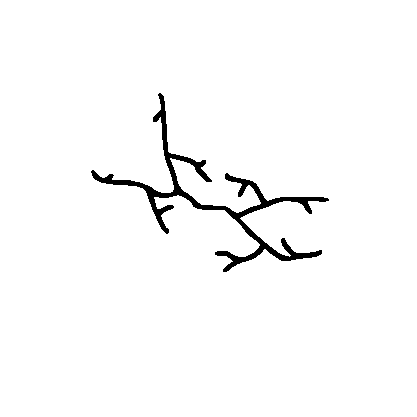
\includegraphics[width=4cm]{../C7/ElementA}}
	\hspace{0.75cm}
	\subfloat[$\hgu = 25$ units]{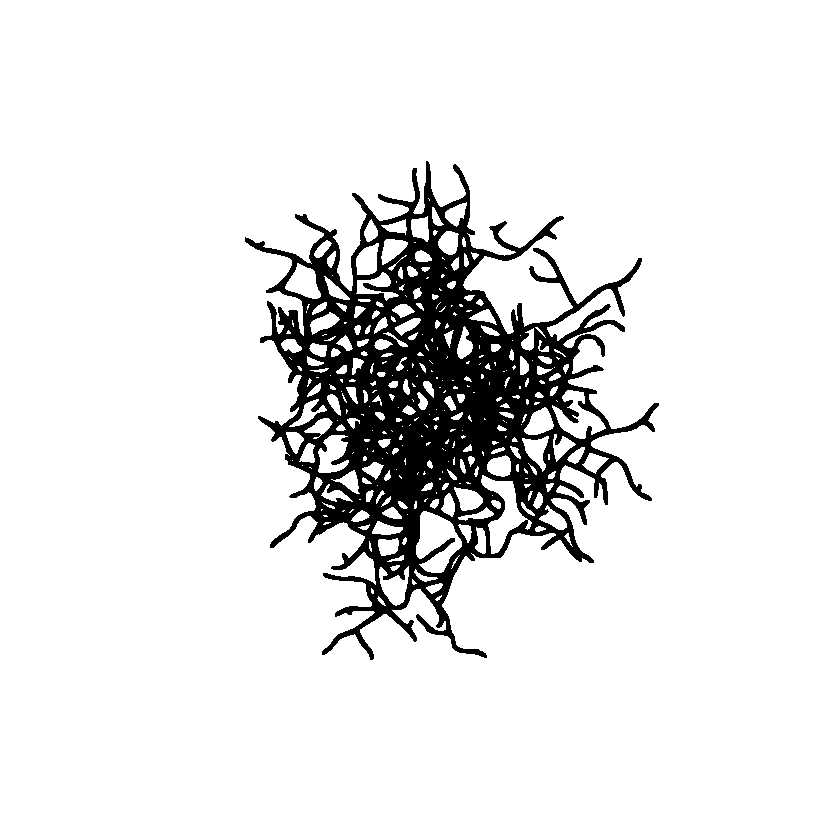
\includegraphics[width=4cm]{../C7/MyceliumA}}
	\hspace{0.75cm}
	\subfloat{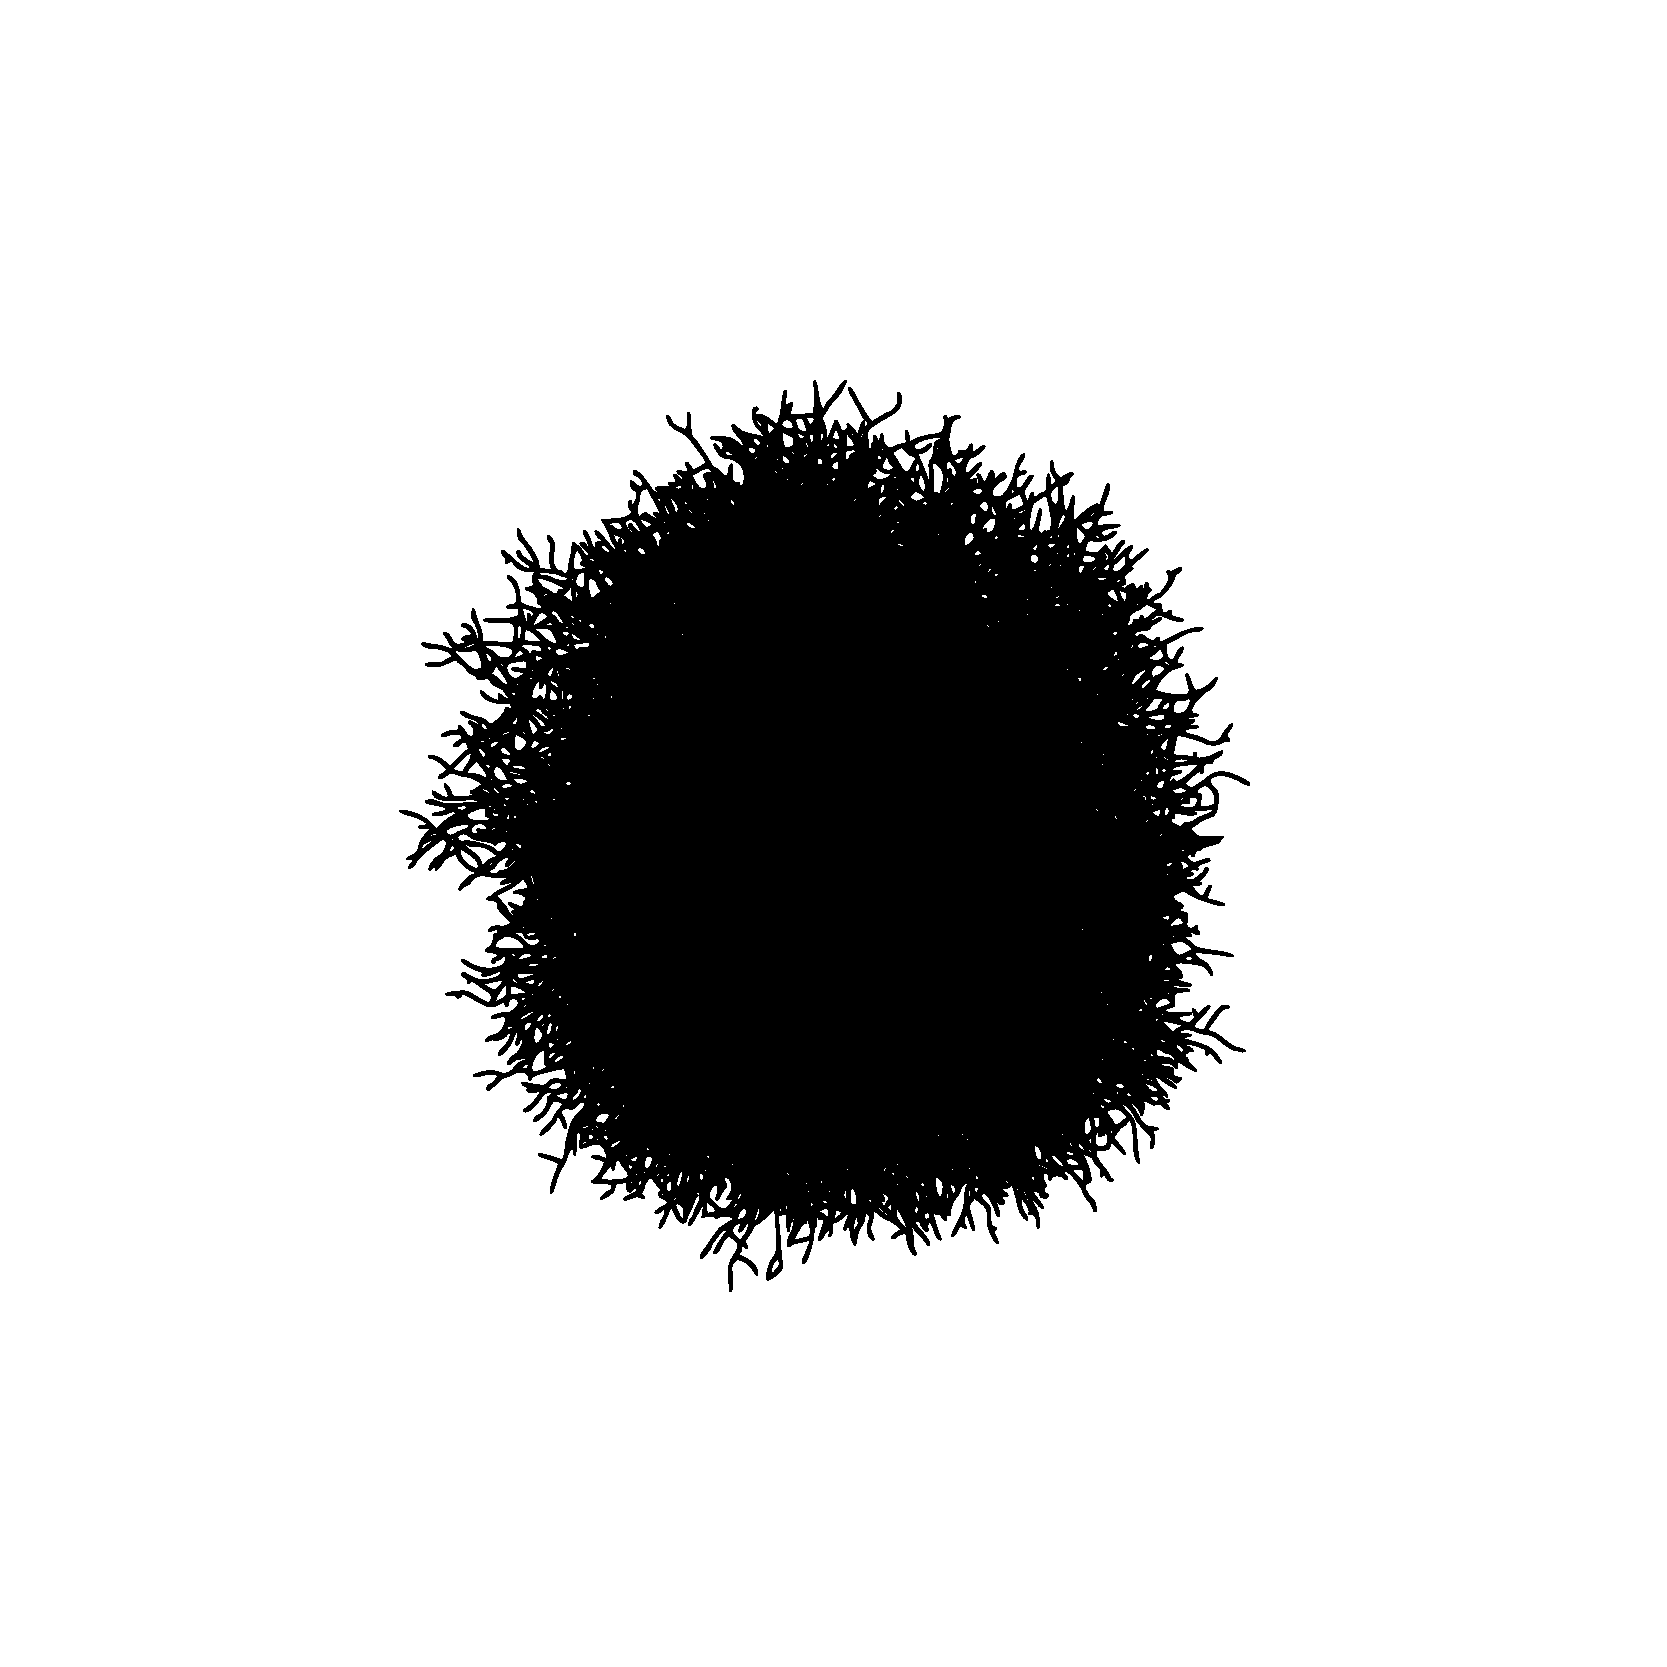
\includegraphics[width=4cm]{../C7/ColonyA}}
	\\
	\subfloat{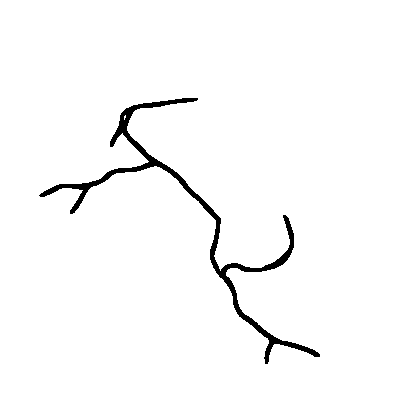
\includegraphics[width=4cm]{../C7/ElementB}}
	\hspace{0.75cm}
	\subfloat[$\hgu = 60$ units]{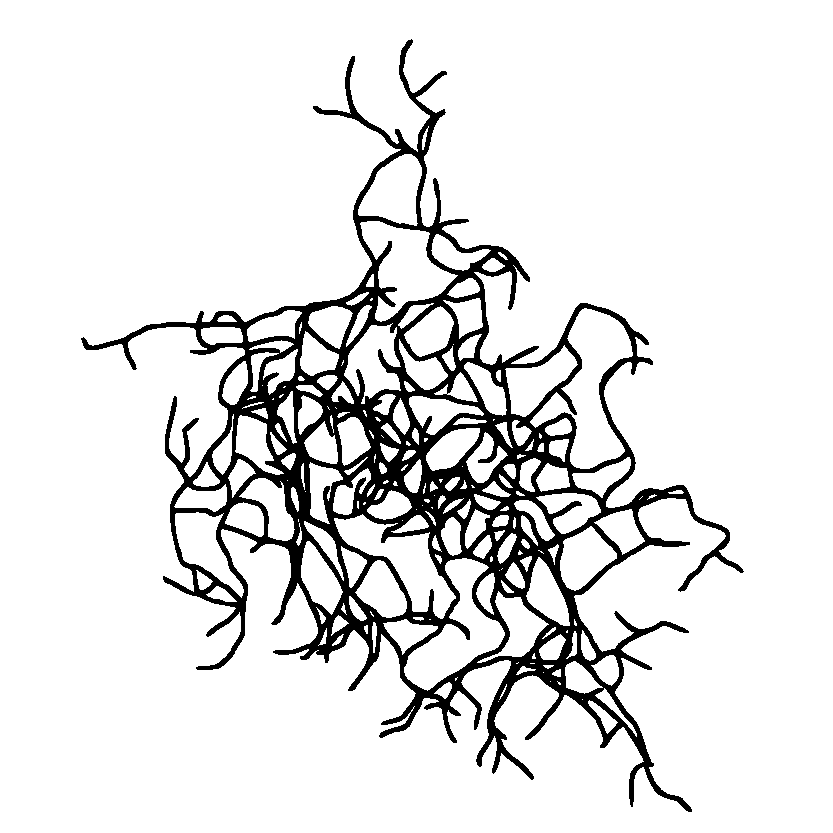
\includegraphics[width=4cm]{../C7/MyceliumB}}
	\hspace{0.75cm}
	\subfloat{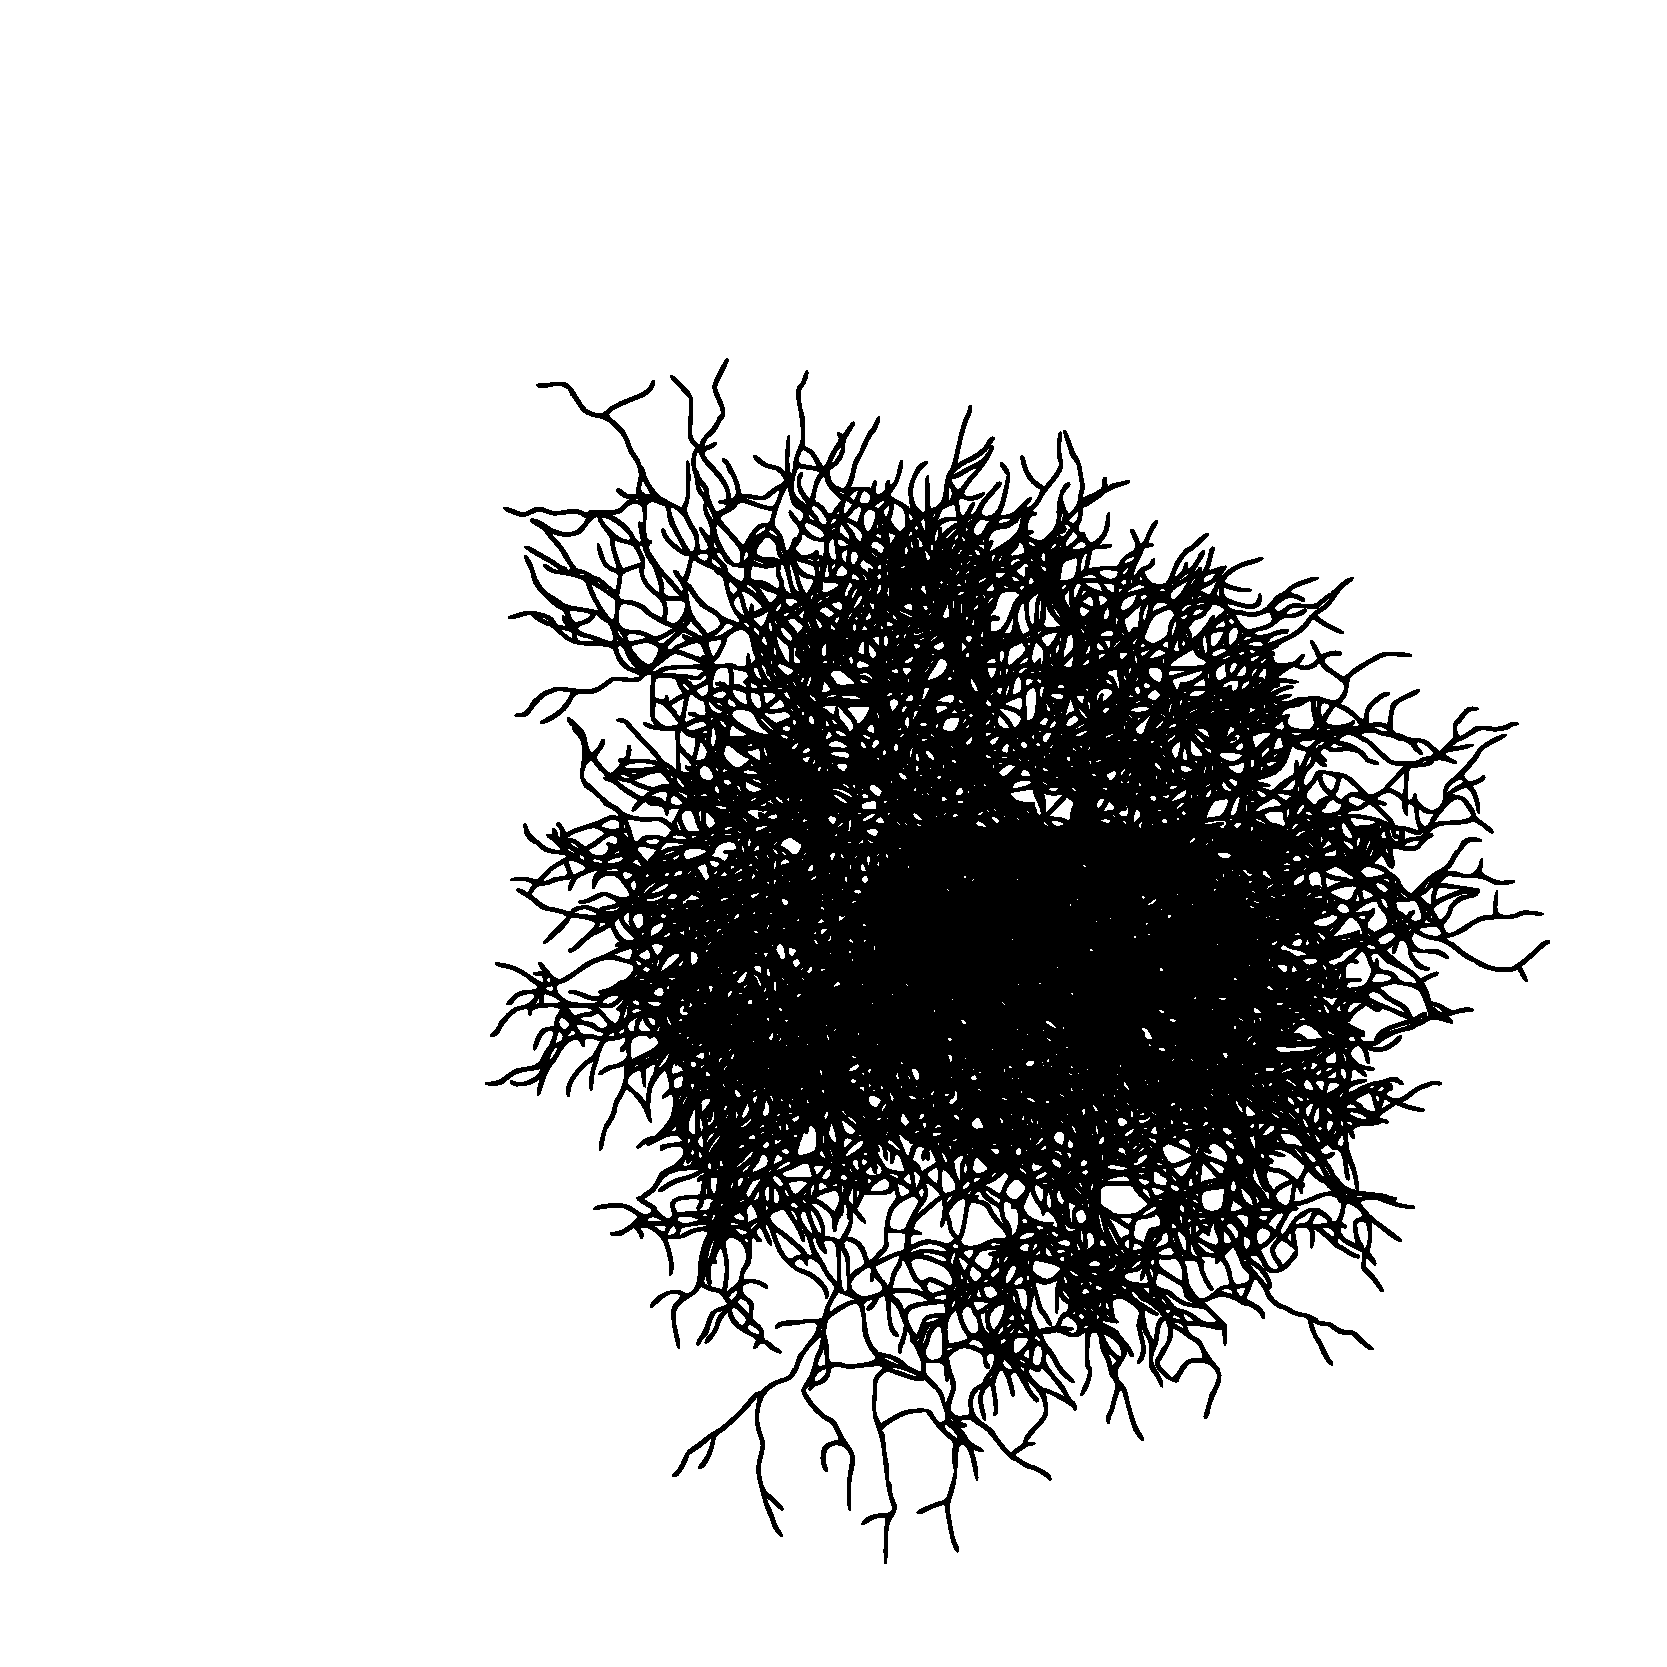
\includegraphics[width=4cm]{../C7/ColonyB}}
	\\
	\subfloat{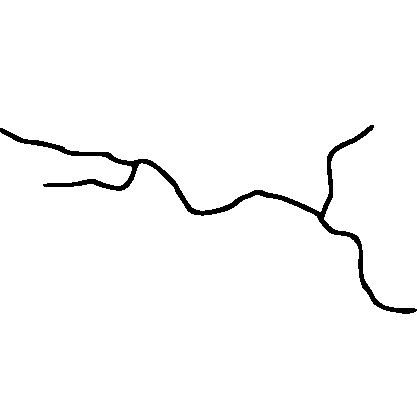
\includegraphics[width=4cm]{../C7/ElementC}}
	\hspace{0.75cm}
	\subfloat[$\hgu = 95$ units]{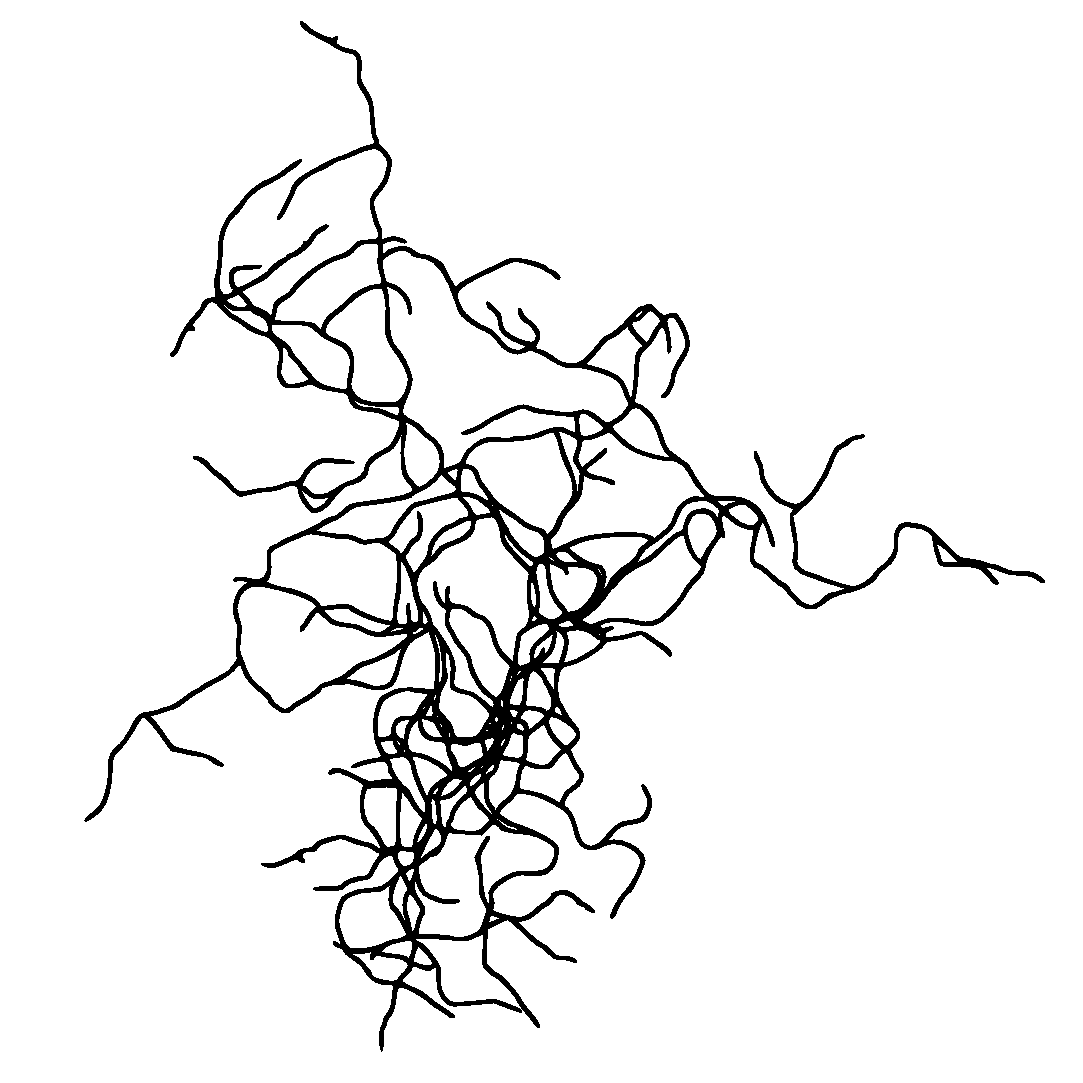
\includegraphics[width=4cm]{../C7/MyceliumC}}
	\hspace{0.75cm}
	\subfloat{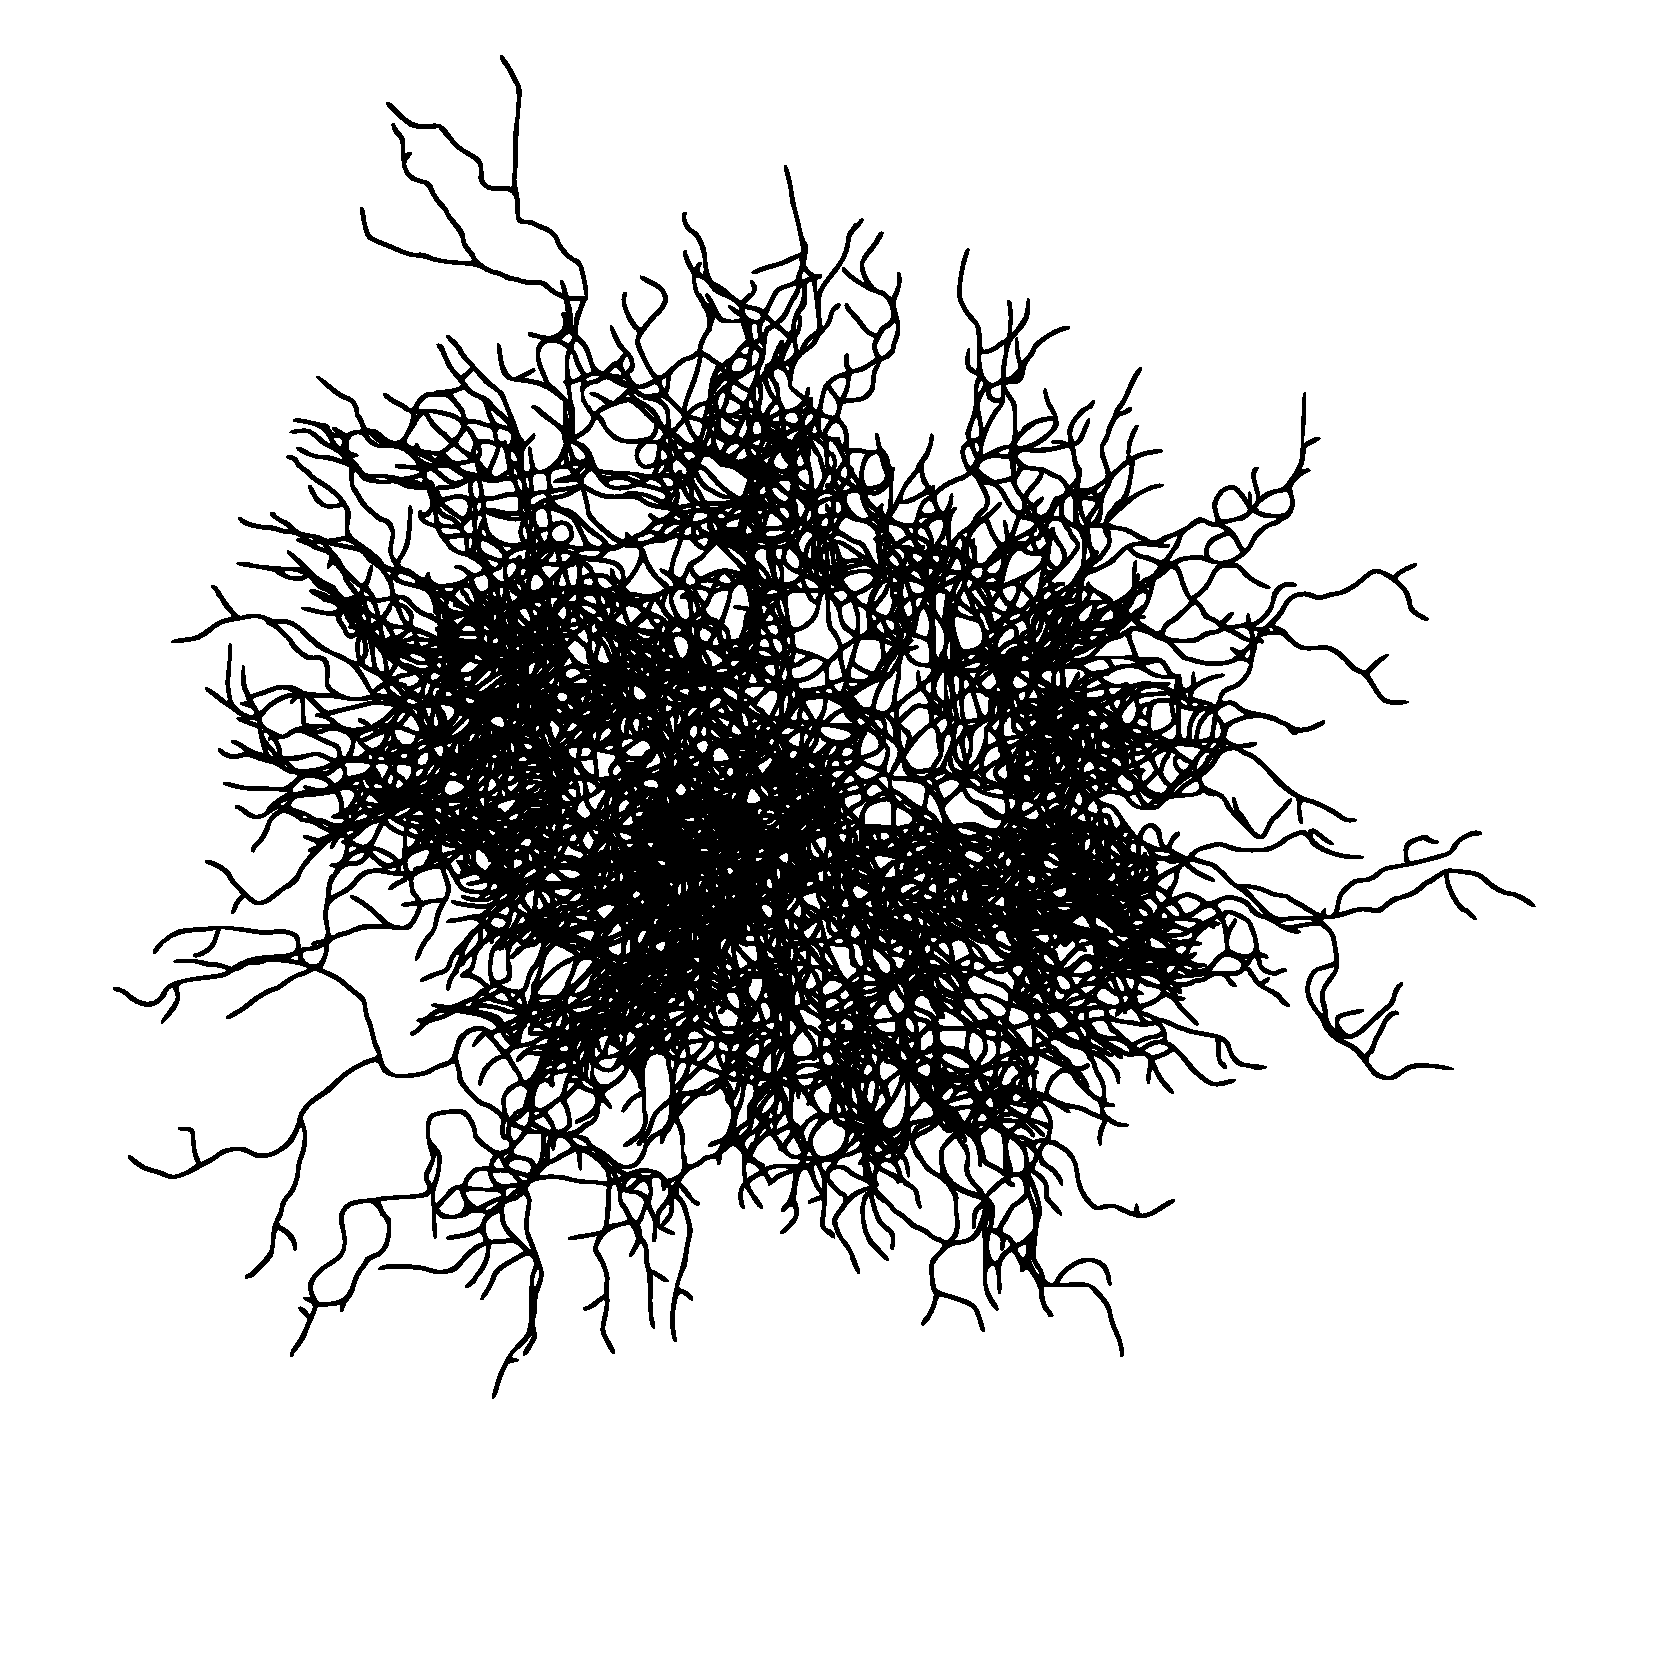
\includegraphics[width=4cm]{../C7/ColonyC}}
	\\
	\subfloat{\pstool[width=(\textwidth - 1cm)]{../C7/TimeAxis}{	\psfrag{T}[Bl][tl]{\bf Time}}}
	\caption{Simulated effect of increasing hyphal growth unit ($\hgu$) on colony macro-morphology.}
	\label{fig:Colonies}
\end{figure}

While it may be possible to relate the hyphal growth unit of \lq young' mycelia cultivated on solid substrates with the fractal dimension of the macroscopic colonies that result, such an investigation must also consider any differing spatial distribution of the different organisms investigated; it is possible that two mycelia can have the same hyphal growth unit while exhibiting different morphological features (Fig.~\ref{fig:GrowthPatterns}). As the directionality of hyphal growth is thought to be determined by concentration gradients in the solid substrate \cite{prosser1995,carlile2001}, cultivation on a membrane placed atop a liquid medium should minimise the impact of this variable and the effect of different medium compositions on hyphal growth unit and, subsequently, colony morphology (fractal dimension) could be examined. However, any differences in foraging strategy (branching angle, for example) would still need to be determined by microscopic assessment. Such an investigation therefore requires the consideration of a large number of variables.

The production of a \lq boundary signal', as used here to evaluate $D$, could also prove useful in cases where the application of a skeletonisation routine to mycelial elements is undesirable; such investigations using image analysis systems may rely on manual tip-counts \cite{muller2003}. However, consider the example presented in Figure~\ref{fig:FracAlg}; it may be possible to identify the hyphal tips as local maxima in the boundary signal. The enumeration of these local turning points could be used as an indicator of tip location in applications where skeletonisation is unsuitable. There also exists the possibility that an examination of object boundaries could prove useful in discriminating between spore clusters and \lq young' hyphae, which can be otherwise morphologically similar (Section~\ref{sec:DevImageAnalDisc}), although it is likely that high-magnification images would be required for such an application to provide sufficiently high resolution, resulting in a significant increase in the time necessary for image capture.

% Improvements to fractal signal method: smoothing of 'signal' for more accurate evaluation of D? Low-pass filtering of sampled signal? Smoothing of spline representing boundary?

Image processing systems represent essential tools for the accurate quantification of fungal morphology, but fully automated systems, designed for this application, are still rare. The system developed in this study has been used in conjunction with a newly-developed immobilisation assay to characterise the growth kinetics of \emph{A. oryzae} on a solid substrate. In addition, published findings on the application of fractal analyses have been expanded upon by relating this parameter to the branching behaviour of the organism using a novel means of fractal dimension evaluation. The growth of \emph{A. oryzae} in shake flask cultures, reports of which are rare in the literature, has also been extensively studied, with data presented on the micro- and macro-morphological form in various different media compositions. The potential exists to combine these research avenues and utilise fractal geometry to further characterise morphological conformations in submerged culture and, subsequently, arrive at a more definitive correlation between phenotypic variation and metabolite production.